\let\negmedspace\undefined
\let\negthickspace\undefined

\documentclass[journal,12pt,onecolumn]{IEEEtran}
%\documentclass[journal,12pt,twocolumn]{IEEEtran}
%
\usepackage{setspace}
\usepackage{gensymb}
%\doublespacing
\singlespacing

%\usepackage{graphicx}
%\usepackage{amssymb}
%\usepackage{relsize}
\usepackage[cmex10]{amsmath}
%\usepackage{amsthm}
%\interdisplaylinepenalty=2500
%\savesymbol{iint}
%\usepackage{txfonts}
%\restoresymbol{TXF}{iint}
%\usepackage{wasysym}
\usepackage{amsthm}
\usepackage{mathrsfs}
\usepackage{txfonts}
\usepackage{stfloats}
\usepackage{cite}
\usepackage{cases}
\usepackage{subfig}
%\usepackage{xtab}
\usepackage{longtable}
\usepackage{multirow}
%\usepackage{algorithm}
%\usepackage{algpseudocode}
\usepackage{enumitem}
\usepackage{mathtools}
\usepackage{tikz}
\usepackage{circuitikz}
\usepackage{verbatim}
\usepackage{hyperref}
%\usepackage{stmaryrd}
\usepackage{tkz-euclide} % loads  TikZ and tkz-base
%\usetkzobj{all}
\usepackage{listings}
\usepackage{color}                                            %%
\usepackage{array}                                            %%
\usepackage{longtable}                                        %%
\usepackage{calc}                                             %%
\usepackage{multirow}                                         %%
\usepackage{hhline}                                           %%
\usepackage{ifthen}                                           %%
%optionally (for landscape tables embedded in another document): %%
\usepackage{lscape}     
\usepackage{multicol}
\usepackage{chngcntr}
\usepackage{iftex}
%\usepackage[latin9]{inputenc}
\usepackage{geometry}
\usepackage{bm}
%\geometry{verbose,tmargin=2cm,bmargin=3cm,lmargin=1.8cm,rmargin=1.5cm,headheight=2cm,headsep=2cm,footskip=3cm}
\usepackage{array}
\newcolumntype{L}[1]{>{\raggedright\let\newline\\\arraybackslash\hspace{0pt}}m{#1}}
\newcolumntype{C}[1]{>{\centering\let\newline\\\arraybackslash\hspace{0pt}}m{#1}}
\newcolumntype{R}[1]{>{\raggedleft\let\newline\\\arraybackslash\hspace{0pt}}m{#1}}

%\usepackage{graphicx}
%\usepackage{setspace}
%\usepackage{parskip}

\def \hsp {\hspace{3mm}}

\makeatletter

\providecommand{\tabularnewline}{\\}



\makeatother
\ifxetex
\usepackage[T1]{fontenc}
\usepackage{fontspec}
%\setmainfont[ Path = fonts/]{Sanskrit_2003.ttf}
\newfontfamily\nakulafont[Script=Devanagari,AutoFakeBold=2,Path = fonts/]{Nakula}
%\newfontfamily\liberationfont{Liberation Sans Narrow}
%\newfontfamily\liberationsansfont{Liberation Sans}
\fi
\usepackage{tikz}
\usepackage{xcolor}
%\usepackage{enumerate}

%\usepackage{wasysym}
%\newcounter{MYtempeqncnt}
\DeclareMathOperator*{\Res}{Res}
%\renewcommand{\baselinestretch}{2}
\renewcommand\thesection{\arabic{section}}
\renewcommand\thesubsection{\thesection.\arabic{subsection}}
\renewcommand\thesubsubsection{\thesubsection.\arabic{subsubsection}}

\renewcommand\thesectiondis{\arabic{section}}
\renewcommand\thesubsectiondis{\thesectiondis.\arabic{subsection}}
\renewcommand\thesubsubsectiondis{\thesubsectiondis.\arabic{subsubsection}}

% correct bad hyphenation here
\hyphenation{op-tical net-works semi-conduc-tor}
\def\inputGnumericTable{}                                 %%

\lstset{
	language=tex,
	frame=single, 
	breaklines=true
}

%\begin{document}
%


\newtheorem{theorem}{Theorem}[section]
\newtheorem{problem}{Problem}
\newtheorem{proposition}{Proposition}[section]
\newtheorem{lemma}{Lemma}[section]
\newtheorem{corollary}[theorem]{Corollary}
\newtheorem{example}{Example}[section]
\newtheorem{definition}[problem]{Definition}
%\newtheorem{thm}{Theorem}[section] 
%\newtheorem{defn}[thm]{Definition}
%\newtheorem{algorithm}{Algorithm}[section]
%\newtheorem{cor}{Corollary}
\newcommand{\BEQA}{\begin{eqnarray}}
	\newcommand{\EEQA}{\end{eqnarray}}
\newcommand{\define}{\stackrel{\triangle}{=}}
\bibliographystyle{IEEEtran}
%\bibliographystyle{ieeetr}
\providecommand{\mbf}{\mathbf}
\providecommand{\pr}[1]{\ensuremath{\Pr\left(#1\right)}}
\providecommand{\qfunc}[1]{\ensuremath{Q\left(#1\right)}}
\providecommand{\sbrak}[1]{\ensuremath{{}\left[#1\right]}}
\providecommand{\lsbrak}[1]{\ensuremath{{}\left[#1\right.}}
\providecommand{\rsbrak}[1]{\ensuremath{{}\left.#1\right]}}
\providecommand{\brak}[1]{\ensuremath{\left(#1\right)}}
\providecommand{\lbrak}[1]{\ensuremath{\left(#1\right.}}
\providecommand{\rbrak}[1]{\ensuremath{\left.#1\right)}}
\providecommand{\cbrak}[1]{\ensuremath{\left\{#1\right\}}}
\providecommand{\lcbrak}[1]{\ensuremath{\left\{#1\right.}}
\providecommand{\rcbrak}[1]{\ensuremath{\left.#1\right\}}}
\theoremstyle{remark}
\newtheorem{rem}{Remark}
\newcommand{\sgn}{\mathop{\mathrm{sgn}}}
\providecommand{\abs}[1]{\left\vert#1\right\vert}
\providecommand{\res}[1]{\Res\displaylimits_{#1}} 
\providecommand{\norm}[1]{\left\lVert#1\right\rVert}
%\providecommand{\norm}[1]{\lVert#1\rVert}
\providecommand{\mtx}[1]{\mathbf{#1}}
\providecommand{\mean}[1]{E\left[ #1 \right]}
\providecommand{\fourier}{\overset{\mathcal{F}}{ \rightleftharpoons}}
%\providecommand{\hilbert}{\overset{\mathcal{H}}{ \rightleftharpoons}}
%\providecommand{\system}{\overset{\mathcal{H}}{ \longleftrightarrow}}
\providecommand{\system}[1]{\overset{\mathcal{#1}}{ \longleftrightarrow}}
\providecommand{\gauss}[2]{\mathcal{N}\ensuremath{\left(#1,#2\right)}}
%
%\newcommand{\solution}[2]{\textbf{Solution:}{#1}}
\newcommand{\solution}{\noindent \textbf{Solution: }}
\newcommand{\cosec}{\,\text{cosec}\,}
\newcommand{\sinc}{\,\text{sinc}\,}
\newcommand{\rect}{\,\text{rect}\,}
\providecommand{\dec}[2]{\ensuremath{\overset{#1}{\underset{#2}{\gtrless}}}}
\newcommand{\myvec}[1]{\ensuremath{\begin{pmatrix}#1\end{pmatrix}}}
\newcommand{\mydet}[1]{\ensuremath{\begin{vmatrix}#1\end{vmatrix}}}
\newcommand*{\permcomb}[4][0mu]{{{}^{#3}\mkern#1#2_{#4}}}
\newcommand*{\perm}[1][-3mu]{\permcomb[#1]{P}}
\newcommand*{\comb}[1][-1mu]{\permcomb[#1]{C}}
%\numberwithin{equation}{section}
\numberwithin{equation}{section}
%\numberwithin{problem}{section}
%\numberwithin{definition}{section}
\makeatletter
\@addtoreset{figure}{problem}
\makeatother
%\let\StandardTheFigure\thefigure
\let\vec\mathbf
%\renewcommand{\thefigure}{\theproblem.\arabic{figure}}
\renewcommand{\thefigure}{\arabic{section}.\arabic{figure}}
%\setlist[enumerate,1]{before=\renewcommand\theequation{\theenumi.\arabic{equation}}
	%\counterwithin{equation}{enumi}
	%\renewcommand{\theequation}{\arabic{subsection}.\arabic{equation}}
\let\StandardTheFigure\thefigure
	\vspace{3cm}
	%\usepackage{babel}
	\begin{document}
		\title{ Logistic Regression }
		\maketitle
		\author{ Mannem Charan AI21BTECH11019}
		\begin{abstract}
			This report consists of my basic understanding of one of the popular Ml methods "Logistic Regression".
		\end{abstract}
		\section{Logistic Regression}
		Logistic Regression is a ML model which adds probability into the discussion.It comes under Supervised learning, a subcategory of machine learning where the dataset has labels and it will form a model which try to predict labels of new input data.\\
		\section{When we should use this?}
		Logistic Regression is employed to predict how likely a binary outcome(0 or 1) can be observed given an input data.Basically it means that our dependent variable$\brak{y}$ has only two outcomes possible, for example, a patient has cancer or not,kohli hits a century or not,whether iam able to complete this report in time or not.So eventhough logistic regression try to predict a real number$\brak{probability}$,it is fair to say that it is used for doing binary classification(a task of classifying the input data into two groups/classes).
		\section{How we will do this?}
		Similar to linear regression first we will try to find $y$ value from the linear combination of weights and input parameters.The difference between linear and logistic is in linear we want to predict the $y$ value itself but in logistic we will modelled the output being 0 or 1 rather a numeric value.We will use $h$ as linear combination of weights and input parameters since we used notation $y$ as a final label of input data. 
		\begin{align}
			h &= w_{1}x_{1} + w_{2}x_{2} + w_3x_3 +.......+w_mx_m + \theta 
		\end{align}
		where $\brak{w_1,w_2,..,w_m}$ are the weights of input vector $\brak{x_1,x_2,..x_m}$ with $m$ be the no. of features(a necessary parameter to predict the output)\\
		$\theta$ is the bias(this factor is used shift the curve up and down like an intercept of a line) 
		\section{The sigmoid function}	 
		Now to get the probability from this $h$ one can use many function but the popular one is sigmoid function,i.e.,
		\begin{align}
			\pr{h} = \frac{1}{1 + e^{-h}}\label{eq:2}
		\end{align}
		Now we will see the graph of sigmoid function,
		\begin{figure}
			\centering
			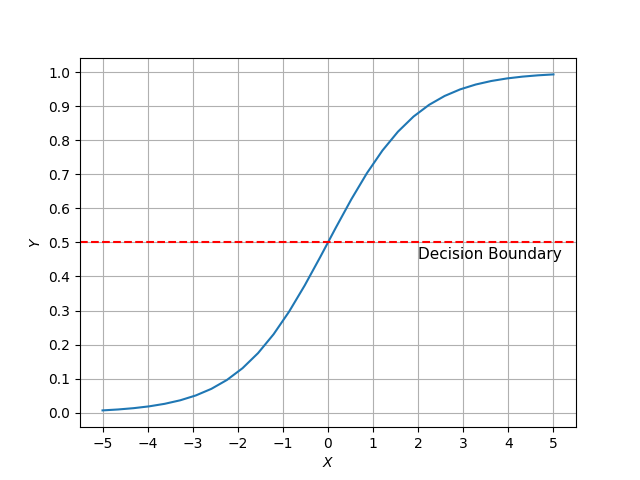
\includegraphics[width=10cm]{sigmoid.png}
			\caption{The sigmoid function}
			\label{Fig:1}
		\end{figure}
		As we can see the output we are getting is in between 0 to 1 and for $h > 0$ the value is greater than .5 and for $h<0$ the value is less than .5.So if we manage to get $h>0$ whenever the input label is 1, we can correlate this sigmoid output value as the probability of getting label 1.So with the $\pr{h} >0.5$ we will predict label as 1 and for $\pr{h}<0.5$ we will predict label as 0.So our main task here is to modify the weights and labels in such a way that $h>0$ whenever the true label is 1 and $h<0$ whenever the true label is 0.   
		\section{Cost Function}
		As you already realised we always to want minimize the error in predicting the label while modifying weights and bias.But in this case,it is not quite similar to what we did in linear regression.\\
		Now lets put our heads straight,are main goal is to make $\pr{h\brak{x}}$ close to 1 when the actual label of $x$ is 1 similarly close to 0 when the actual label of $x$ is 0.It is similar to say that we want to make maximize $\log\brak{\pr{h\brak{x}}}$ when the label of $x$ $\brak{y}$ is 1 since $\log$ is monotonic function but real reason that we are using it will be discussed in your higher classes just kidding!! , we will discuss that in gradient descent section.\\
		So coming to the topic, it is similar to say that we want minimize $-\log\brak{\pr{h\brak{x}}}$, the thing is whenever we say cost function we want to minimize that,so the overall cost function for a input vector $x$ looks like,
		\begin{align}
			J\brak{x} &= \begin{cases}
				-\log\brak{\pr{h\brak{x}}} &, when y = 1\\
				-\log\brak{1 - \pr{h\brak{x}}} &, when y = 0
			\end{cases}
		\end{align}
		The same thing can be written as,
		\begin{align}
			J\brak{x} &= -y\log\brak{\pr{h\brak{\vec{w},\theta}}} - \brak{1-y}\log\brak{\pr{h\brak{\vec{w},\theta}}}
		\end{align}
		Here I changed $h\brak{x}$ to $h\brak{\vec{w},\theta}$ because they are the actual parameters and this notation useful for later purpose.\\
		Now for a dataset $\brak{\vec{x_i},y_i}_{i=1}^{N}$, the cost function looks like,
		\begin{align}
			J &= \frac{1}{N}\brak{\sum_{i=1}^{N}-y_{i}\brak{\log\brak{\pr{h_i\brak{\vec{w},\theta}}} - \brak{1-y_i}\log\brak{\pr{h_i\brak{\vec{w},\theta}}}}}
		\end{align}
		Now we will try to minimize the cost function gradient descent method.
		\section{Gradient Descent}
		Before going to the method, first we will compare it with linear regression. The cost function of it looks like,
		\begin{align}
			J &= \sum_{i=1}^{N}\frac{\brak{Y_i -y_i}^{2}}{2}\\
			&= \sum_{i=1}^{N}\frac{\brak{Y_i-\brak{\vec{w}^TX+\theta}}}{2}
		\end{align}
		Now if we plotted the graph w.r.t weights and J it looks like Fig $\ref{Fig:2}$,\\
		\begin{figure}
			\centering
			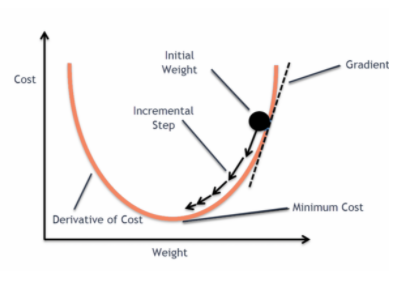
\includegraphics[width=10cm]{convex.png}
			\caption{convex curve}
			\label{Fig:2}
		\end{figure}
		As you can see since it is convex graph using gradient descent method is effective, we will move down to minima of cost function in each step. Now in the case of logistic, if we don't use log of $\pr{h\brak{\vec{w},\theta}}$,the plot between J and weights looks like,$\ref{Fig:3}$\\
		\begin{figure}
			\centering
			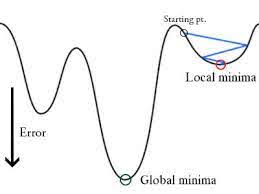
\includegraphics[width=8cm]{non_convex.jpg}
			\caption{Non convex}
			\label{Fig:3}
		\end{figure}
		As you can see since their are many local minima, the gradient descent method may fail to reach the global minima it entirely depends on the starting weight.That the reason why we replace it with log term. 
		\begin{figure}
			\centering
			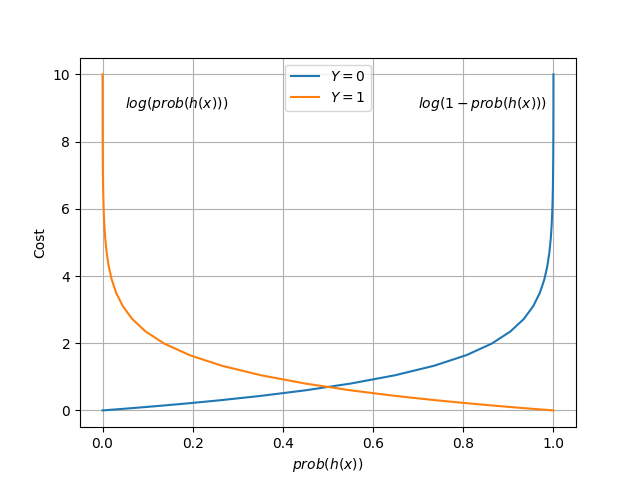
\includegraphics[width=15cm]{logi_cost.png}
			\caption{$prob(h(x))$ vs cost}
			\label{Fig:4}
		\end{figure}
		As we can see here, for $y=1$ if probability tends to 1 the cost tend to 0 and if probability tends to 0 the cost tends to infinity.Similar resemblance can be seen for $y=0$.
		This makes easier for gradient descent method to reach the minimum.So in each iteration we will modify the weights and bias with $\alpha$ as learning rate as,
		\begin{align}
			\vec{w_k} &= \vec{w_k} -\alpha \frac{\partial J}{\partial w_k}\label{eq:9}\\
			\theta_k &= \theta_k - \alpha \frac{\partial J}{\partial \theta_k}\label{eq:10}
		\end{align}
		where $w_k$ and $\theta_k$ are weight vector and bias after $k^{th}$ iteration.
		Now we will understand $\eqref{eq:9}$, let say $\vec{w} =\myvec{w_1\\w_2\\w_3\\.\\.\\w_m}$, now we want to modify each of these weights in a iteration, to do that
		first we will simplify the cost function,
		\begin{align}
			J &= \frac{1}{N}\brak{\sum_{i=1}^{N}-y_{i}\log\brak{\pr{h_i\brak{\vec{w},\theta}}} - \brak{1-y_i}\log\brak{\pr{h_i\brak{\vec{w},\theta}}}}
		\end{align}
		Using $\eqref{eq:2}$,
		\begin{align}
			J &= \frac{1}{N}\brak{\sum_{i=1}^{N}-y_{i}\log\brak{\frac{1}{1+e^{-h_i}}} - \brak{1-y_i}\log\brak{1-\frac{1}{1+e^{-h_i}}}}\\
			&= \frac{1}{N}\brak{\sum_{i=1}^{N}y_{i}\log\brak{1+e^{-h_i}} + \brak{1-y_i}\log\brak{1+e^{h_i}}}
		\end{align}
		Now if we do the paritial derivative w.r.t $w_j$ where $j \in \cbrak{1,2,...m}$,
		\begin{align}
			\frac{\partial J}{\partial w_j} &= \frac{1}{N}\brak{\sum_{i=1}^{N}y_{i}\frac{1}{1+e^{-h_i}}-e^{-h_i}\frac{\partial h_i}{\partial w_j} + \brak{1-y_i}\frac{1}{1+e^{h_i}}e^{h_i}\frac{\partial h_i}{\partial w_j}}\label{eq:14} 
		\end{align}
		Now we know that,
		\begin{align}
			h_i &= \vec{w^T}\vec{x_i} + \theta \\
			&= w_1x_{1i} + w_2x_{2i} + ..+w_jx_{ji}.. w_mx_{mi} + \theta\\
			\frac{\partial h_i}{\partial w_j} &= x_{ji}\label{eq:17}
		\end{align}
		Here the notation $x_{ji}$ can be understood as the $j^{th}$ feature of $i^{th}$ input vector.
		Using $\eqref{eq:17}$,we can modify $\eqref{eq:14}$ as,
		\begin{align}
			\frac{\partial J}{\partial w_j} &= \frac{1}{N}\brak{\sum_{i=1}^{N}y_i\frac{-1}{e^{h_i} + 1}x_ji + \brak{1-y_i}\frac{e^{h_i}}{1+e^{h_i}}x_ji}\\
			&= \frac{1}{N}\brak{\sum_{i=1}^{N}x_{ji}\brak{y_i\brak{-1} + \frac{1}{1 + e^{-h_i}}}}\\
			&= \frac{1}{N}\brak{\sum_{i=1}^{N}x_{ji}\brak{-y_i + \pr{h_i}}}\\
			&= \frac{1}{N}\brak{\sum_{i=1}^{N}x_{ji}\brak{\pr{h_i}-y_i}}
		\end{align}
		So with $\alpha$ as learning rate we will modify each weight in $k^{th}$ iteration as shown below,
		\begin{align}
			w_{1k} &= w_{1k} - \alpha\frac{1}{N}\brak{\sum_{i=1}^{N}x_{1i}\brak{\pr{h_i}-y_i}}\\
			w_{2k} &= w_{2k} - \alpha\frac{1}{N}\brak{\sum_{i=1}^{N}x_{2i}\brak{\pr{h_i}-y_i}}\\
			& ...\nonumber \\
			& ...\nonumber\\
			w_{mk} &= w_{mk} - \alpha\frac{1}{N}\brak{\sum_{i=1}^{N}x_{mi}\brak{\pr{h_i}-y_i}}
		\end{align}
		Similarly solving $\eqref{eq:10}$ gives,
		\begin{align}
			\theta_k = \theta_k - \alpha\frac{1}{N}\sum_{i=1}^{N}\brak{\pr{h_i} - y_i}
		\end{align}
		In this way we will modify weights and bias over the iterations in gradient descent method.
		\section{Regularization}
		Similar to linear regression, logistic regression also requires regularisation since it also assumes linear relationship(with a non-linear transform of output).
		The goal of regularization is to minimize the generalization error without effecting the training error.Often, the model tend to learn too perfectly which leads
		to problem of overfitting.To avoid that we add square of norm of $\beta$ to the cost function.
		\begin{align}
			\beta &= \myvec{\vec{w}\\\theta}
		\end{align}
		This shrinks the weights/coefficients of the model without disturbing the training error of the model.This is necessary because in our data there may lie some o
		utliers which may helps the model more flexible (outliers are data points which don't follow normal trend) but at the risk of overfitting.\\
		The new cost function looks like,
		\begin{align}
			J &= \frac{1}{N}\brak{\sum_{i=1}^{N}-y_{i}\brak{\log\brak{\pr{h_i\brak{\vec{w},\theta}}} - \brak{1-y_i}\log\brak{\pr{h_i\brak{\vec{w},\theta}}}}} +
			\lambda\norm{\beta}^2
		\end{align}
		where, $\lambda$ is a tuning factor which decides how much we want penalize the flexibility of the model.
		\section{Summary}
		In this report we discussed about,
		\begin{enumerate}
			\item What is logistic regression?
			\item When we should use logistic regression?
			\item The cost function of logistic regression
			\item The gradient descent method for logistic regression.
			\item Regularization of the model
		\end{enumerate}
		\section{Questions}
		\begin{enumerate}
			\item How logistic regression is different from linear regression?.
			\item Why do we need bias term in logistic regression?
			\item Can you think of a function which can do same job as sigmoid function?
			\item How the value of learning rate affects the training of the model?
			\item How regularization is justified?
		\end{enumerate}
	\end{document}
